\documentclass[a4paper,11pt]{article}
\usepackage[a4paper,bindingoffset=0.2in,left=1in,right=1in,top=1in,bottom=1in,footskip=.25in]{geometry}
\usepackage{graphicx}
\usepackage[none]{hyphenat}
\usepackage[a4paper]{geometry}
\usepackage{enumerate}
\newgeometry{left=2cm,bottom=2cm,right=2cm}

\title{Functional Specification, E-R Model, Test Plan, Schema Design and Screen Design for Database and Information Systems Project}

\begin{document}
\maketitle
\section{Introduction}
This document describes the functional specifications, the E-R model and the Test plan of the application being developed to meet the requirements of the completion of the Database and Information Systems Lab project. The project details are as below: 
\begin{itemize}
\item Name of the Project : \emph{Trawell}
\item Team Members : Mridul Garg (110050030), Anand Soni (110050037), Sanchit Garg (110050035), Himanshu Roy (110050019) 
\end{itemize}

\section{Project Domain}
\begin{itemize}
\item Tourism. The application will serve as a travel planner and guide for tourists. 
\end{itemize}

\section{Application Specifications}
Based on the category of the user, the application is supposed to provide the following functionalities:
\begin{itemize}
\item For an unregistered user : An unregistered user is any random visitor who comes across and explores the application.
\begin{itemize}
\item Search for tourist places by country, state or city
\item Search for a tourist place by its name
\end{itemize}
\item For a registered user : A registered user is one who has filled in her personal details and has been provided login credentials.
\begin{itemize}
\item Search for tourist places by country, state or city
\item Search for a tourist place by its name
\item Search for hotels by city or tourist spot
\item Search for speciality cuisines of the region
\item Rate places visited and hotels stayed in
\item See the places and hotels that she has rated 
\item Maintain a wishlist for the places she wants to visit
\item Prepare and modify a travel plan for her tour
\item Maintain a history which records all the details of her trip
\item Delete history items
\item Maintain a manual schedule as against the plan
\item Update personal information
\end{itemize}
\item For Administrators : An administrator is the owner of this application who can create and modify the database and can also add more users to it (employees or customers).
\begin{itemize}
\item Modify the tourism database
\item Create logins for recruited employees
\end{itemize}
\item For employees : An employee (not necessarily a user) has the power to modify the database.
\begin{itemize}
\item Modify the tourism database
\end{itemize}
\end{itemize}

\section{Aspects Modelled}
As a part of this application, we have created 10 entities and modelled them as below:
\begin{itemize}
\item Modelled Customers, Administrator, Countries, States, Cities, Tourist spots, Hotels, Schedule.
\item Modelled travel plan, user's tour history. 
\end{itemize}

\section{Aspects Not Modelled}
The following aspects have not been modelled in the application:
\begin{itemize}
\item Review system, Festivals, Shopping, Entertainment and other activities.
\end{itemize}

\section{Role of Each Member}
This section roughly describes the parts of the project that each member will contribute to. However, the actual contributions may differ.
\begin{itemize}
\item Mridul Garg
\begin{itemize}
\item Design of the Functional Specification
\item Design of relational database and screen
\item Normalization and design of final schema
\item Writing SQL scripts for schema and other programming tasks.
\end{itemize}
\item Anand Soni
\begin{itemize}
\item Design of the Functional Specification
\item E/R modelling and creation of test plan 
\item Design of relational database and screen
\item Writing SQL scripts for schema and other programming tasks.
\end{itemize}
\item Sanchit Garg
\begin{itemize}
\item Design of the Functional Specification
\item E/R modelling and creation of test plan
\item Normalization and design of final schema
\item Writing SQL scripts for schema and other programming tasks.
\end{itemize}
\item Himanshu Roy
\begin{itemize}
\item Design of the Functional Specification
\item E/R modelling and creation of test plan
\item Normalization and design of final schema
\item Writing SQL scripts for schema and other programming tasks.
\end{itemize}
\end{itemize}

\section{Possible Value Addition}
The following features might prove to be further value additions to this project which we have not planned to model/implement:
\begin{itemize}
\item Hotel Bookings
\item Travel Bookings and planning
\end{itemize}

\section{The E-R Model}
\begin{figure}[ht!]
\centering
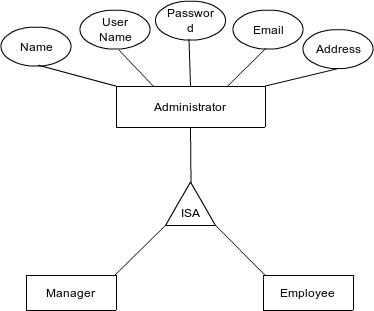
\includegraphics[width=80mm]{admin.png}
\caption{E-R Model}
\label{overflow}
\end{figure}

\begin{figure}[ht!]
\centering
\makebox[\textwidth]{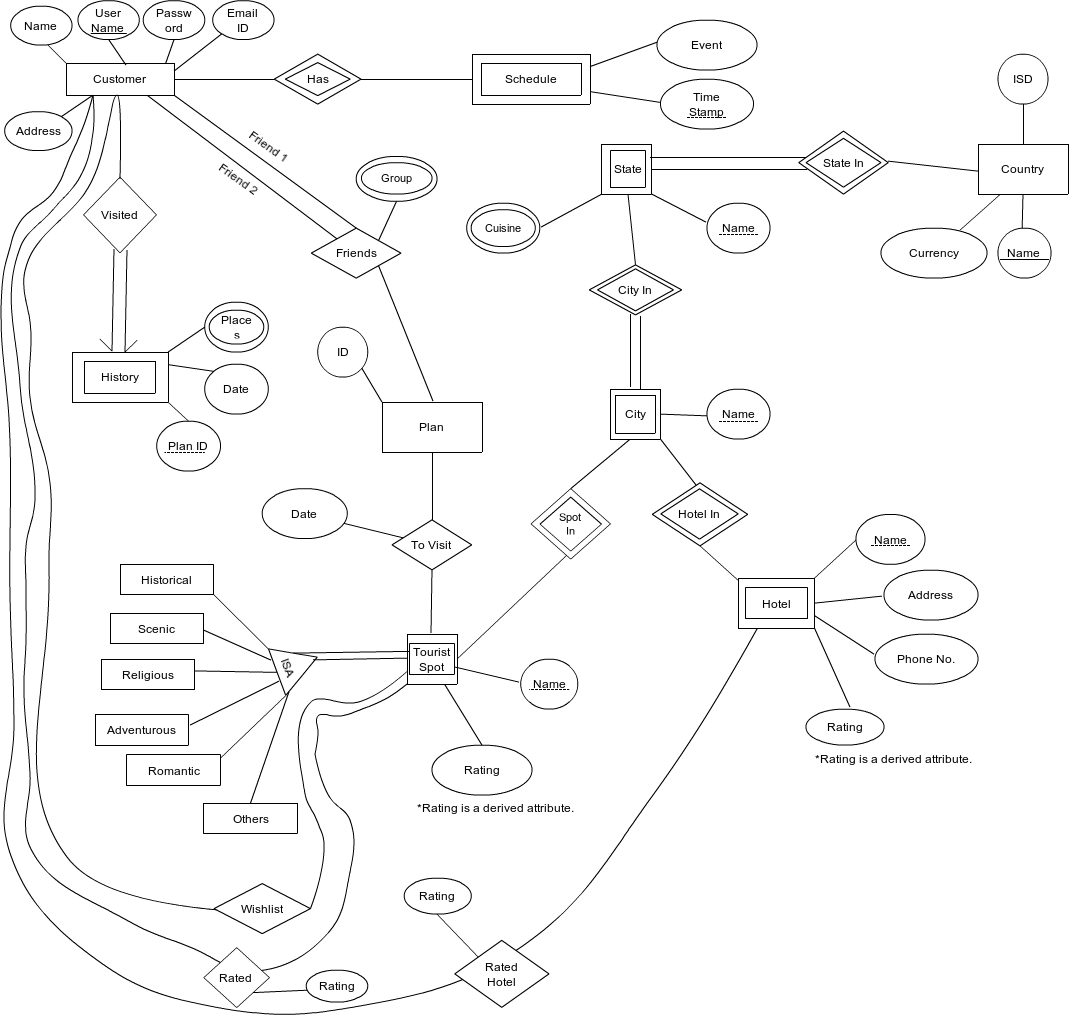
\includegraphics[width=\paperwidth]{er.png}}
%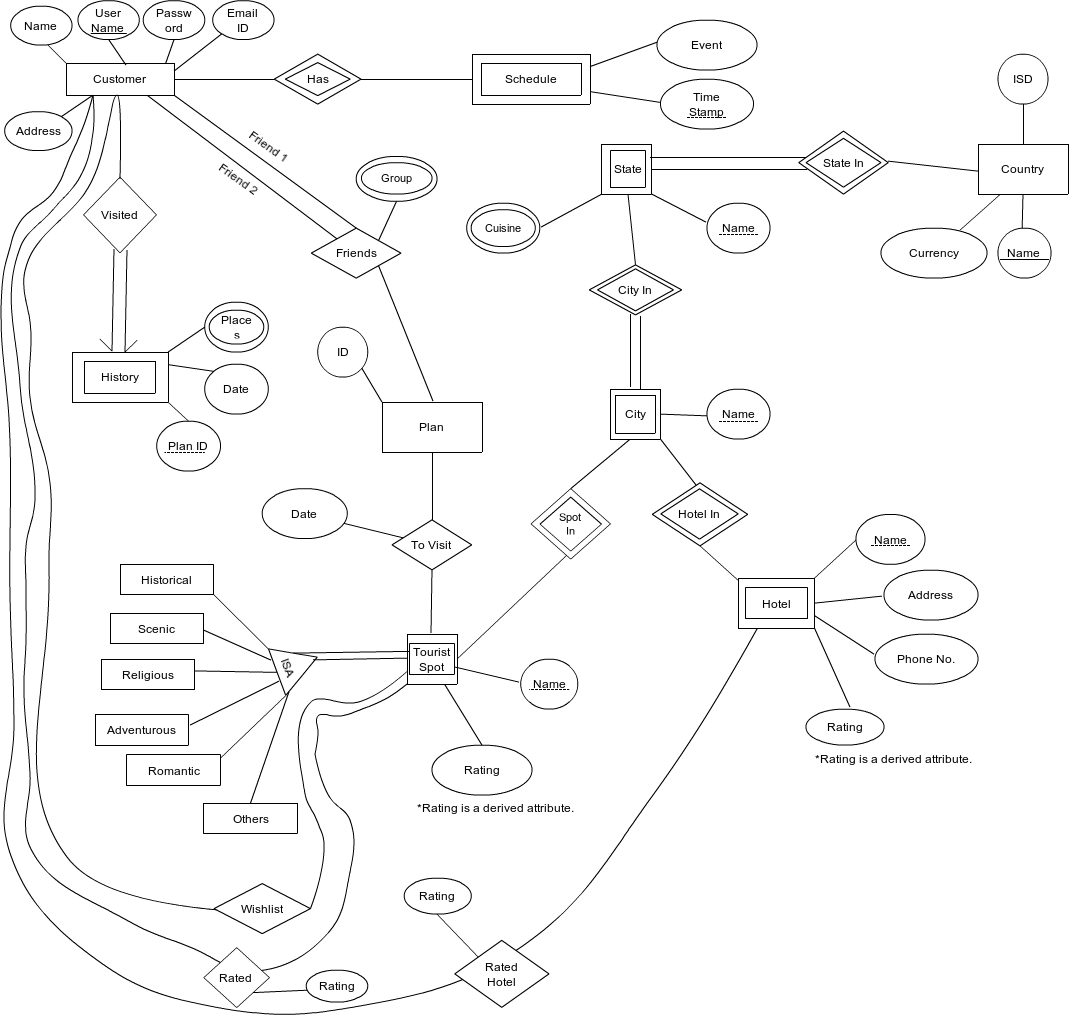
\includegraphics[width=200mm]{er.png}
\caption{E-R Model}
\label{overflow}
\end{figure}
.
\newline
\newline
\newline
\newline
\section{Test Plan}
\begin{itemize}
\item Search for a tourist place by country, state or city :
\newline
In this case, no edge cases need to be taken care of as the user is not allowed to query manually.

\item Search for a tourist place by its name :
\newline
If the user enters a wrong name (one that does not exist in the database),  we will redirect her to an error page showing the name entered is invalid. This page will have an option to go back to the search page.

\item Search for hotels by city or tourist spot :
\newline
If the user enters a wrong hotel name (one that does not exist in the database corresponding to the place or city),  we will redirect her to an error page showing the name entered is invalid. This page will have an option to go back to the search page.

\item Search for speciality cuisines of the region :
\newline
In this case, we will show her the cuisine results only for that particular region (no option to manually search will be provided to the user). Hence, no exceptions to handle.

\item Rate places visited and hotels stayed in :
\newline
If a user decides not to rate a hotel or place, there should not be an error. The rating will be on a scale of 10. Also, same user will not be allowed to rate a place or hotel multiple times. 

\item Maintain and modify a wishlist for the places (tourist spot) she wants to visit :
\newline
On delete of a particular entry from wishlist, the remaining entries in the wishlist should remain intact.

\item Prepare and modify a travel plan for her tour :
\newline
In case of a group travel plan (Friends plan), if a particular customer modifies her plan, the plan must be automatically updated in the other friends' plans too. Plan must be consistent for all users. 
\newline
If two users attempt to modify group travel plan, it must not be allowed. We will use synchronization for this.

\item Add a user to a group plan :
\newline
If a customer is added to a group plan without her permission, she must not be added to the plan. Repeated addition of the same customers will throw an error message.

\item Maintain a history which records all the details of her trip :
\newline
Since history is never manually modified, no boundary cases will come up.

\item Update personal information :
\newline
While updating email address, if the customer enters an already existing email id, she will be prompted to enter the email address again. Also, if she leaves blank the cells corresponding to name, password or email id, we will ask her to enter valid entries.

\item Modify the tourism database (for administrator and employees) :
\newline
If the admin deletes a city from a database, the corresponding tourist spots should also be deleted. All dependencies must be dealt with properly.
\newline
If a new city is added by an employee and it already exists in the database, we will prompt her with an error.

\item Create logins for recruited employees (for administrator) :
\newline
Similar to point Update personal information.

\item Updating/creating/maintaining plan :
\newline
Date and time of a new plan, if given before the current time, the user should be prompted with an error and asked to enter a valid time/date.

\end{itemize}

\section{Schema Design, Screen Design, Functional Dependencies and Assertions}
\subsection{Schema Design}
\subsubsection{Entities}

\begin{itemize}
\item Country(Name PRIMARY KEY, Currency, ISD)
\item State(Country(Reference to Country.Name), Name(Discriminator), Cuisine, STDCode)
\item City(Country(Reference to Country.Name), State , Name(Discriminator), Pincode UNIQUE)
\item Customer(Username PRIMARY KEY, Name NOT NULL, Password NOT NULL, EmailID NOT NULL, Address)
\item Schedule(CustomerID (Reference to Customer.Username),Event NOT NULL, TimeStamp(Discriminator) NOT NULL)
\item History(CustomerID (Reference to Customer.Username), PlanID (DISCRIMINATOR), Date NOT NULL, PlaceID NOT NULL)
\item HistoryPlaces(PlaceID(Reference to History.PlaceID), CountryName(Reference to Country.Name), StateName , CityName , SpotName(Reference to TouristSpotName))
\item Plan(ID PRIMARY KEY)
\item Hotel(CountryName(Reference to Country.Name), StateName , CityName , HotelName(Discriminator), Address NOT NULL, PhoneNo., NumberOfHits, Rating)
\end{itemize}

\subsubsection{IS-A Relationships}
\begin{itemize}
\item For Administration
\begin{itemize}
\item E/R Approach
\begin{itemize}
\item Administrator(Name NOT NULL, Username PRIMARY KEY, Password NOT NULL, Role NOT NULL, EmailID , Address)
\item Manager(ID (Reference to Administrator.Username))
\item Employee(ID (Reference to Administrator.Username))
\end{itemize}
\item OO Approach
\begin{itemize}
\item Administrator(Name NOT NULL, Username PRIMARY KEY, Password NOT NULL, Role NOT NULL, EmailID , Address)
\item Manager(Name NOT NULL, Username PRIMARY KEY, Password NOT NULL, Role NOT NULL, EmailID , Address)
\item Employee(Name NOT NULL, Username PRIMARY KEY, Password NOT NULL, Role NOT NULL, EmailID , Address)
\end{itemize}
\end{itemize} 
\item For Tourist-Spot
\begin{itemize}
\item E/R Approach
\begin{itemize}
\item TouristSpot(CountryName(Reference to Country.Name), StateName , CityName , Name(Discriminator), Rating, Description)

\item Historical(CountryName(Reference to Country.Name), StateName , CityName , SpotName(Discriminator), YearReference)
\item Scenic(CountryName(Reference to Country.Name), StateName , CityName , SpotName(Discriminator))
\item Historical(CountryName(Reference to Country.Name), StateName , CityName , SpotName(Discriminator), Religion)
\item Adventurous(CountryName(Reference to Country.Name), StateName , CityName , SpotName(Discriminator), AdventureType)
\item Others(CountryName(Reference to Country.Name), StateName , CityName , SpotName(Discriminator), Speciality NOT NULL)

\end{itemize}
\item OO Approach \newline
As we have 5 subclasses for TouristSpot Class, here for sake of convenience and readability we are describing only some of the relations, like
\begin{itemize}
\item Historical(CountryName(Reference to Country.Name), StateName , CityName , SpotName(Discriminator), YearReference, Rating, Description)
\item HistReli(CountryName(Reference to Country.Name), StateName , CityName , SpotName(Discriminator), YearReference, Religion, Rating, Description)
\item AdvenHistScenic(CountryName(Reference to Country.Name), StateName , CityName , SpotName(Discriminator), AdvcentureType, YearReference, Rating, Description)
\item And many more
\end{itemize}
\end{itemize}
\end{itemize}

\subsubsection{Many-to-many Relationships}
Here in our Database there are only many-to-many relationships that are "Friends" and "ToVisit", "RatedHotel", "RatedSpot" and "Wishlist". Here “Plan” Entity is modified as per stated in the problem statement corresponding to many-to-many relationships “Friends” and “ToVisit” . Above “Plan” Entity should be ignored. Also "Customer" Relation is also modified corresponding to "Wishlist","RatedSpot" and "RatedHotel". Above "Plan" and “Customer” Entities should be ignored.
\begin{itemize}
\item Plan(CustomerID(Reference to Customer.Username), PlanID, GroupID NOT NULL, Date NOT NULL, CountryName(Reference to Country.Name), StateName , CityName , SpotName(Reference to TouristSpotName)). NumberofGroup corresponds to multi-attribute field

\item Group(GroupID(Reference to Friends.GroupID), Friend(Reference to Customer.ID))

\item Customer(Username PRIMARY KEY, Name NOT NULL, Password NOT NULL, EmailID NOT NULL, Address, EmailID NOT NULL, RSCityName(Referenced to City.Name), RSStateName(Referenced to State.Name), RSCountryName(Referenced to Country.Name), SpotName(Referenced to TouristSpot.Name), SRating, RHCityName(Referenced to City.Name), RHStateName(Referenced to State.Name), RHCountryName(Referenced to Country.Name), HotelName(Referenced to Hotel.Name), HRating, WCityName(Referenced to City.Name), WStateName(Referenced to State.Name), WCountryName(Referenced to Country.Name), WSpotName(Referenced to TouristSpot.Name))
\end{itemize}

\subsection{Assertions}
\begin{itemize}
\item STD codes for different states are different in a country.
\item Pincodes are different for different cities in a country.
\item In the Schedule/Plan relation a user can update/enter event corresponds to  only after the current timestamp.
\item Rating of a hotel or a tourist spot should be consistent with the rating data on updation of it’s rating by the user. i.e. the current rating should be updated if a user update or rate a spot or hotel.
\end{itemize}

\subsection{Functional Dependecies}
\begin{itemize}
\item For Customer Relation
\begin{itemize}
\item Username $\rightarrow$ password, name, EmailID, Address.
\item EmailID $\rightarrow$ Username
\end{itemize}

\item For History Relation 
\begin{itemize}
\item PlanID, Username $\rightarrow$ PlaceID, Date
\end{itemize}

\item For Schedule Relation
\begin{itemize}
\item Username, TimeStamp $\rightarrow$ Event
\end{itemize}
\item For Country Relation
\begin{itemize}
\item Name $\rightarrow$ Currency, ISD
\end{itemize}
\item For State Relation
\begin{itemize}
\item CountryName, StateName $\rightarrow$ Cuisine
\end{itemize}
\item For City Relation
\begin{itemize}
\item CountryName, StateName, CityName $\rightarrow$ CountryName, StateName, CityName 
\end{itemize}
\item For Hotel Relation
\begin{itemize}
\item CountryName, StateName, CityName,HotelName $\rightarrow$ Address,PhoneNo., Rating, NumberOfHits 
\end{itemize}
\item For RatedHotel Relation
\begin{itemize}
\item CountryName, StateName, CityName,HotelName,Username $\rightarrow$ Rating
\end{itemize}
\item For TouristSpot Relation
\begin{itemize}
\item CountryName, StateName, CityName, Name $\rightarrow$ Rating, NumberOfHits,
\item Given Cusatomer.Username $\rightarrow$ WishlistID
\item CustomerID, CountryName, StateName, CityName, TouristSpot.Name $\rightarrow$ User.SpotRating, Description
\item CustomerID, CountryName, StateName, CityName, Hotel.Name $\rightarrow$ User.HotelRating
\end{itemize}
\item For Plan Relation
\begin{itemize}
\item CustomerID, PlanID $\rightarrow$ GroupID
\item PlanID, Date $\rightarrow$ SpotID
\end{itemize}
\end{itemize}

\subsection{Normalization}
\begin{itemize}
\item Customer(Username PRIMARY KEY, Name NOT NULL, Password NOT NULL, EmailID NOT NULL, Address, EmailID NOT NULL, RSCityName(Referenced to City.Name), RSStateName(Referenced to State.Name), RSCountryName(Referenced to Country.Name), SpotName(Referenced to TouristSpot.Name), SRating, RHCityName(Referenced to City.Name), RHStateName(Referenced to State.Name), RHCountryName(Referenced to Country.Name), HotelName(Referenced to Hotel.Name), HRating, WCityName(Referenced to City.Name), WStateName(Referenced to State.Name), WCountryName(Referenced to Country.Name), WSpotName(Referenced to TouristSpot.Name)). \newline \newline
We have the following FD’s from the above relation :
\begin{itemize}
\item Username $\rightarrow$ Name, Password, Address, EmailID
\item Username,RSCityName, RSStateName, RSCountryName, SpotName $\rightarrow$ SpotRating
\item Username, RHCityName, RHStateName, RHCountryName, HotelName $\rightarrow$ HotelRating
\item Username, WCityName, WStateName, WCountryName $\rightarrow$ WSpotName
\end{itemize}
Now we can see that not a single FD is trivial and none of the LHS of the FD is super-key, this implies that the above relation is not in BCNF. Following the rules for BCNF decomposition, we get the following to relations :
\begin{itemize}
\item R1(Username, Password, Name, Address, EmailID)
\item R2(RSCityName, RSStateName, RSCountryName, SpotName, SRating, RHCityName, RHStateName, RHCountryName, HotelName, HRating, WCityName, WStateName, WCountryName, WSpotName).
\end{itemize}
Now R2 is not in BCNF while R1 is. FD no.1 is still preserved. Applying BCNF decomposition to R2 based on FDs no. 2,3,4, altogether we get four relations, which are:
\begin{itemize}
\item R1(Username, Password, Name, Address, EmailID)
\item R2(Username, RSCityName, RSStateName, RSCountryName, SpotName, SRating)
\item R3(Username, RHCityName, RHStateName, RHCountryName, HotelName, HRating)
\item R4(Username, WCityName, WStateName, WCountryName, WSpotName)
\end{itemize}

Since  all the FDs remain preserved after this decomposition, we need not revert to 3NF as there are no added redundancies. Also there is no need for 4NF decomposition.

\item Plan(CustomerID(Reference to Customer.Username), PlanID, GroupID NOT NULL, Date NOT NULL,  CountryName(Reference to Country.Name), StateName , CityName , SpotName(Reference to TouristSpotName)). \newline
*GroupID corresponds to multi attribute field.\newline \newline
We have the following FDs from the above relation :
\begin{itemize}
\item CustomerID, PlanID $\rightarrow$ GroupID
\end{itemize}

Now, since the FD is not trivial and nor is (CustomerID, PlanID) a super-key for the relation, we can decompose it to BCNF. Following the rules for BCNF decomposition, we get the following to relations :
\begin{itemize}
\item R1(CustomerID, PlanID, GroupID).
This relation is consistent with the ‘friends’ relation in our E/R model and is in BCNF.
\item R2(CustomerID, PlanID, CountryName, StateName, CityName, SpotName, Date).
\end{itemize}

In this relation there are no non-trivial FD’s possible as the super-key consists of all the attributes of the relation taken together. Thus, we have one trivial FD. Hence, this relation too is in BCNF. R2 corresponds with ToVisit relation in the E/R model. \newline
Since  all the FD’s remain preserved after this decomposition, we need not revert to 3NF as there are no added redundancies. \newline
We have the following multivalued dependencies from R2 :
\begin{itemize}
\item CustomerID, PlanID, Date $\rightarrow$ CountryName, StateName, CityName, SpotName
\end{itemize}

This FD implies that for a given (CustomerID, PlanID, Date) tuple, a customer can have many (CountryName, StateName, CityName, SpotName) tuples. He can visit many places on a given date in a given plan. Now, we apply the 4NF decomposition algorithm to this FD. We get the following relations:
\begin{itemize}
\item R3(CustomerID, PlanID, Date , CountryName, StateName, CityName, SpotName). R3 is obviously in 4NF.
\item R4(CustomerID, PlanID, Date, GroupID). For R2, we have only trivial FD’s. Hence, R4 too is in 4NF.
\end{itemize}
However, breaking into R3 and R4 reduces no redundancy, infact, redundancy is increased and hence, this 4NF decomposition is trivial. We conclude that R2 is in 4NF too. \newline
\end{itemize}

\subsubsection*{Further Modifications}
The E/R diagram shows an IS-A relation for the TouristSpot entity. We have modified this. Since a tourist spot can be under more than one IS-A categories, a lot of redundancies will creep in once we build the database. Hence, for the sake of efficient design, we have introduces a ‘Type’ multivalued attribute for the ‘Tourist Spot’ entity. This will contain names of all the former IS-A categories where that particular spot falls like Historical or Religious or Historical and Religious.

\subsection{Final Schema Design}
Following are the schemas which we are going to use in the project
\begin{itemize}
\item Country(\underline{Name}, Currency, ISD)
\item State(\underline{Country FOREIGN KEY Country.Name), Name}, Cuisine, STDCode)
\item City(\underline{ID AUTO INCREMENT},Country(FOREIGN KEY Country.Name), State(FOREIGN KEY State.Name) , Name, Pincode )
\item TouristSpot(\underline{City.ID, SpotName}, Rating, Description, TypeID NOT NULL)
\item TouristSpotType(TypeID NOT NULL, Type(1 or more than 1 combination of 'Historical', 'Adventerous', 'Religious' and 'Scenic' or 'Other'))
\item Customer(\underline{Username}, Password, Name, Address, EmailID)
\item Administrator(\underline{Username}, Password, Name, Address, EmailID, Role('Manager' or 'Employee'))
\item Schedule(\underline{Username(FOREIGN KEY Customer.Username), TimeStamp}, Event NOT NULL)
\item History(\underline{CustomerID(FOREIGN KEY Customer.Username), PlanID, Date}, PlaceID NOT NULL)
\item HistoryPlaces(PlaceID(FOREIGN KEY History.PlaceID), City.ID , SpotName(FOREIGN KEY TouristSpot.Name))
\item Plan(\underline{ID})
\item SpotRating(Username(FOREIGN KEY Customer.Username), CityID(FOREIGN KEY City.ID), SpotName (FOREIGN KEY TouristSpot.Name), SRating)
\newline \textbf{*Primary Key :- Username, CityID, SpotName}
\item HotelRating(Username(FOREIGN KEY Customer.Username), CityID(FOREIGN KEY City.ID), HotelName, HRating)
\newline \textbf{*Primary Key :- Username, CityID, HotelName}
\item WishList(Username(FOREIGN KEY Customer.Username), CityID(FOREIGN KEY City.ID), WSpotName(FOREIGN KEY TouristSpot.Name))
\item ToVisit(CustomerID(FOREIGN KEY Customer.username), PlanID(FOREIGN KEY Plan.ID), CityID(FOREIGN KEY City.ID), SpotName(FOREIGN KEY TouristSpot.Name), Date).
\item Friends(\underline{CustomerID(FOREIGN KEY Customer.username), PlanID(FOREIGN KEY Plan.ID)}, GroupID)
\item Group(GroupID(FOREIGN KEY Friends.GroupID), Friend(FOREIGN Key Customer.ID))
\item Hotel(CityID(FOREIGN KEY City.ID), HotelName, Address NOT NULL, PhoneNo NOT NULL, NumberOfHits NOT NULL, Rating NOT NULL)
\end{itemize}

\subsection{Screen Design}
%Screen Design are to be found in "screendesign-2013-10-13.zip" in the folder.
\begin{figure}[ht!]
\hfill\includegraphics[width=170mm]{./screen_design/home.png}\hspace*{\fill}
\caption{Home Screen}
\end{figure}

\begin{figure}[ht!]
\hfill\includegraphics[width=170mm]{./screen_design/login.png}\hspace*{\fill}
\caption{Login page}
\end{figure}

\begin{figure}[ht!]
\hfill\includegraphics[width=170mm]{./screen_design/signup.png}\hspace*{\fill}
\caption{Registration page}
\end{figure}

\begin{figure}[ht!]
\hfill\includegraphics[width=170mm]{./screen_design/afterlogin.png}\hspace*{\fill}
\caption{Logged In page}
\end{figure}

\begin{figure}[ht!]
\hfill\includegraphics[width=170mm]{./screen_design/country.png}\hspace*{\fill}
\caption{Search by country $\rightarrow$ Results}
\end{figure}

\begin{figure}[ht!]
\hfill\includegraphics[width=170mm]{./screen_design/aftercountry.png}\hspace*{\fill}
\caption{Search by state of the country selected}
\end{figure}

\begin{figure}[ht!]
\hfill\includegraphics[width=170mm]{./screen_design/state.png}\hspace*{\fill}
\caption{States of selected country}
\end{figure}

\begin{figure}[ht!]
\hfill\includegraphics[width=170mm]{./screen_design/city.png}\hspace*{\fill}
\caption{Popular cities of the state selected}
\end{figure}

\begin{figure}[ht!]
\hfill\includegraphics[width=170mm]{./screen_design/aftercity.png}\hspace*{\fill}
\caption{Popular Tourist Spots \& Hotels of the selected city}
\end{figure}

\begin{figure}[ht!]
\hfill\includegraphics[width=170mm]{./screen_design/rating.png}\hspace*{\fill}
\caption{Description of the selected Spot or Hotel}
\end{figure}

\begin{figure}[ht!]
\hfill\includegraphics[width=170mm]{./screen_design/profile.png}\hspace*{\fill}
\caption{User Profile}
\end{figure}

\begin{figure}[ht!]
\hfill\includegraphics[width=170mm]{./screen_design/currentplan.png}\hspace*{\fill}
\caption{Current plans of the User}
\end{figure}

\begin{figure}[ht!]
\hfill\includegraphics[width=170mm]{./screen_design/plantravel.png}\hspace*{\fill}
\caption{Add a new Plan}
\end{figure}

\begin{figure}[ht!]
\hfill\includegraphics[width=170mm]{./screen_design/history.png}\hspace*{\fill}
\caption{History of the travel of the User}
\end{figure}

\begin{figure}[ht!]
\hfill\includegraphics[width=170mm]{./screen_design/wishlist.png}\hspace*{\fill}
\caption{User's Wishlist}
\end{figure}
\end{document}
